%% COMPILER AVEC XELATEX

\documentclass[11pt, a4paper]{article}
\usepackage[french]{babel}
%\usepackage[utf8]{inputenc}
\usepackage{fontspec,xunicode}
\setromanfont{Linux Biolinum O} %% POLICE REQUISE
%\usepackage[T1]{fontenc}

\usepackage{geometry}
\geometry{hmargin=2cm, vmargin=2.5cm} %%% Marges

\usepackage{fancyhdr}
\pagestyle{fancy}
\fancyhf{}
\lhead{Sécurité 2012-2013}
\rhead{M2 MIAGE - Université d'Orléans}
\rfoot{\thepage/\pageref{lastpage}}
%\lfoot{Version $\alpha$}%\footnotesize\url{http://www.univ-orleans.fr/lifo/Members/Bastien.Le-gloannec/ChallengeCrypto/}

%\usepackage{amsmath,amssymb}
\usepackage{amsmath}
\usepackage{graphicx,xcolor,tikz}
\usepackage{enumerate,url,hyperref,subfigure}
\usepackage[geometry]{ifsym}

%%%%%%%%%%%%%%%%%%%%%%%%%%%%%%%%%%%%%%%%%%%%%%%%%%%%%%%%%%%%%%%%%%%%%%%%
\begin{document}

\newcommand{\TODO}{\textcolor{red}{\framebox{\textbf{TODO}}}}

%%%%%%%%%%%%%%%%%%%%%%%%%%%%%%%%%%%%%%%%%%%%%%%%%%%%%%%%%%%%%%%%%%%%%%%%

\newcommand{\titre}[1]{\begin{center}\Huge\textbf{#1}\end{center}}

\newcommand{\newexo}[3]{\paragraph{#1}{\small#2}\hfill{}{\textit{#3}}}

\newcommand{\superfantome}{\vphantom{abcdefghijklmnopqrstuvwxyz0123456789ABCDEFGHIJKLMNOPQRSTUVWXYZ\_}}

\newcommand{\codebox}[1]{\raisebox{-0.135cm}{\tikz{\node[fill=blue!10,rounded
      corners,inner sep=2pt]{\small\tt\superfantome#1};}}}


%% NB : largeur voulue des grandes box : textwidth + 8pt (4pt de chaque côté)

\newcommand{\groupe}[1]{
  \vspace{0.6cm}%
  \noindent\hspace{-4pt}%
  \tikz{\node[fill=black!70, rounded corners, inner sep=4pt]{\makebox[\textwidth]{\color{white}\textbf{\superfantome#1}}};}%
  \vspace{-0.3cm}%
}

%% Correction de la largeur pour inner sep 6pt (au lieu de 4pt)
\newlength{\boxwidth}
\addtolength{\boxwidth}{\textwidth}
\addtolength{\boxwidth}{-4pt}

\newcommand{\bigbox}[2]{\noindent\hspace{-4pt}\tikz{\node[fill=#1,rounded
    corners,inner sep=6pt]{\parbox{\boxwidth}{#2}};}}

\newcommand{\bigbluebox}[1]{\bigbox{blue!10}{#1}}
\newcommand{\bigredbox}[1]{\bigbox{red!10}{#1}}
\newcommand{\biggreenbox}[1]{\bigbox{green!10}{#1}}

\newcommand{\centercodebox}[1]{
  \begin{center}%
  \tikz{\node[fill=blue!10,rounded corners,inner sep=6pt]{\parbox{0.8\textwidth}{\tt #1}};}%
  \end{center}%
}

\newcommand{\pictotriangle}{\textcolor{red!60}{\raisebox{-1.2pt}{\FilledTriangleUp}}}
\newcommand{\pictocarre}{\textcolor{green!50}{\raisebox{-2pt}{\FilledSquare}}}
\newcommand{\pictocercle}{\textcolor{blue!60}{\raisebox{-1.5pt}{\FilledCircle}}}

\tikzstyle{polygonstyle}=[draw=black!70,fill=black!50,line width=1pt]
\newcommand{\polygona}{\tikz[scale=0.1]{\filldraw[polygonstyle] (0.00000,1.00000) -- (-0.86603,-0.50000) -- (0.86603,-0.50000)  --cycle;}}
\newcommand{\polygonb}{\tikz[scale=0.1]{\filldraw[polygonstyle] (0.00000,1.00000) -- (-1.00000,0.00000) -- (-0.00000,-1.00000) -- (1.00000,-0.00000)  --cycle;}}
\newcommand{\polygonc}{\tikz[scale=0.1]{\filldraw[polygonstyle] (0.00000,1.00000) -- (-0.95106,0.30902) -- (-0.58779,-0.80902) -- (0.58779,-0.80902) -- (0.95106,0.30902)  --cycle;}}
\newcommand{\polygond}{\tikz[scale=0.1]{\filldraw[polygonstyle] (0.00000,1.00000) -- (-0.86603,0.50000) -- (-0.86603,-0.50000) -- (-0.00000,-1.00000) -- (0.86603,-0.50000) -- (0.86603,0.50000)  --cycle;}}
\newcommand{\polygone}{\tikz[scale=0.1]{\filldraw[polygonstyle] (0.00000,1.00000) -- (-0.78183,0.62349) -- (-0.97493,-0.22252) -- (-0.43388,-0.90097) -- (0.43388,-0.90097) -- (0.97493,-0.22252) -- (0.78183,0.62349)  --cycle;}}
\newcommand{\polygonf}{\tikz[scale=0.1]{\filldraw[polygonstyle] (0.00000,1.00000) -- (-0.70711,0.70711) -- (-1.00000,0.00000) -- (-0.70711,-0.70711) -- (-0.00000,-1.00000) -- (0.70711,-0.70711) -- (1.00000,-0.00000) -- (0.70711,0.70711)  --cycle;}}

\renewcommand{\labelitemi}{\polygonb}  %%% Puce enumerations

\newcommand{\incise}{\scalebox{2.5}[1]{-}}

%%%%%%%%%%%%% D E B U T %%%%%%%%%%%%%%%

\titre{Challenge Cryptanalyse}

\vspace{0.3cm}

\bigbluebox{\pictocercle{}~~Vous avez dû recevoir une archive spécifique à votre
  groupe par mail. Tous les chemins indiqués dans ce sujet sont relatifs à la racine de l'archive.}

\groupe{Deux chiffres historiques}

\newexo{Défi \no1}{}{}\\
Le message \texttt{Defi1/message.txt}, initialement en français, a été chiffré par une méthode élémentaire.
\begin{itemize}
\item[\polygona] Saurez-vous le déchiffrer ?
\end{itemize}

\newexo{Défi \no2}{}{}\\
Le message \texttt{Defi2/message.txt}, initialement en anglais, a été chiffré par une méthode classique à clef, résistante à la cryptanalyse du précédent défi. 
\begin{itemize}
\item[\polygona] Trouvez et implémentez une méthode de cryptanalyse adéquate.
\end{itemize}

\groupe{Enigma}

\vspace{0.7cm}

\biggreenbox{\pictocarre{}~~Une implémentation de la machine Enigma est disponible en Java (dans \texttt{enigma/java}) et en Python (dans \texttt{enigma/python}). Vous utiliserez
indifféremment l'un ou l'autre des langages selon votre préférence. La
machine implémentée est absolument identique dans les deux
langages. Elle comporte 3 rotors, dont l'ordre peut être modifié, et au
plus 6 fiches afin de définir une permutation dans le
\emph{brouilleur} (tableau de
fiches) par échange de lettres.}

\vspace{0.3cm}

\noindent Une \emph{clef} de la machine Enigma
est la donnée de toutes les informations nécessaires pour configurer la
machine afin de crypter/décrypter (cela revient au
même du fait du réflecteur) un message. La clef comporte donc :
l'ordre des rotors, leurs positions initiales et les fiches utilisées
dans le brouilleur.\\\\
Rappelons avant de commencer la structure d'un message
crypté. Tous les opérateurs allemands disposaient d'une même \emph{clef du jour} définie à l'avance et valable une journée donnée. Afin de ne pas
chiffrer tous les messages avec cette même clef (\emph{question
  subsidiaire :} expliquer pourquoi), l'opérateur choisissait avant
l'envoi d'un message un autre jeu de positions initiales pour les
rotors. Il mettait alors sa machine dans la configuration du jour,
tapait la clef choisie deux fois pour prévenir les erreurs (par
exemple, pour les positions $(0,1,2)$, il entrait "ABCABC"), puis
mettait les rotors dans les positions choisies et chiffrait le
message. Ce \emph{préfixe} de 6 caractères a donc un rôle différent et n'est pas chiffré avec la même clef que le corps du message.%\\

\iffalse
\bigbluebox{Une \emph{permutation} est une bijection d'un ensemble dans
  lui-même. Elle admet une unique décomposition en produits de cycles
  à supports disjoints.}\fi

\newexo{Défi \no3}{}{}\\
Les deux messages \texttt{Defi3/message1.txt} et \texttt{Defi3/message2.txt} ont été interceptés par les télécommunications alliées. Nos espions nous informent en outre que la machine utilisée est identique à celle qui vous a été fournie et qu'au plus trois fiches du brouilleur ont été utilisées pour le chiffrement. En revanche, la clef n'est pas connue et est différente pour les deux messages. 
\begin{itemize}
\item[\polygona] Pourrez-vous les cryptanalyser rapidement en exploitant la puissance des ordinateurs d'aujourd'hui ?
\end{itemize}

\newexo{Défi \no4}{}{}\\
Le cryptologue Marian Rejewski fut au début des années 1930 à l'origine de la première (et plus
jolie) avancée dans la cryptanalyse d'Enigma. Exploitant la répétition des clefs choisies au début de chaque message, sa méthode
permettait d'identifier très rapidement un ensemble généralement très
restreint (quelques dizaines) de possibles clefs du jour (hors
brouilleur) après avoir analysé les six premiers caractères de seulement quelques dizaines, voire centaines, de messages interceptés dans la journée.\\
La méthode de Rejewski se base sur des empreintes, extraites des messages
reçus dans la journée, que l'on présentera sous la forme de trois
relations binaires $\overset{\text{1-4}}{\longrightarrow}$,
$\overset{\text{2-5}}{\longrightarrow}$ et $\overset{\text{3-6}}{\longrightarrow}$ liant
respectivement les 1\ier{} et 4\ieme, 2\ieme{} et 5\ieme{}, 3\ieme{}
et 6\ieme{} caractères des préfixes interceptés. Partant initialement
de relations vides, on enrichit nos relations binaires, à chaque préfixe "ABCDEF" intercepté, des associations
A$\overset{\text{1-4}}{\longrightarrow}$ D, B$\overset{\text{2-5}}{\longrightarrow}$ E
et C$\overset{\text{3-6}}{\longrightarrow}$ F. Dès qu'une relation associe
au moins une lettre à chacune des lettres de l'alphabet, on considère sa construction \emph{complète}. Ces trois relations constituent les empreintes extraites par Rejewski.

\bigredbox{\pictotriangle{}~~On pourra supposer dans toute la suite que les Allemands
  ne font jamais de faute de frappe (il n'y a donc jamais
  d'erreur dans le préfixe des messages interceptés) et que
  suffisamment de messages ont été interceptés pour que les empreintes
  soient complètes.}

\vspace{0.3cm}

\noindent Les trois questions théoriques suivantes vous aiderons à comprendre la
méthode de Rejewski. Il n'est \textbf{pas indispensable} d'avoir
traité ces questions avant de passer à l'implémentation de la méthode.

\vspace{0.2cm}

\begin{itemize}
\item[\polygona] Justifier que les trois empreintes extraites par Rejewski forment des
  permutations.\\
  \emph{Indication.}~~Il s'agit pour cela de justifier que les relations
  formées sont bien fonctionnelles (c'est-à-dire qu'à toute lettre est
  associée une unique autre lettre) et bijectives.
\item Considérant deux permutations $\sigma$ et $\alpha$, quelle
  permutation obtient-on en composant
  $\sigma'=\alpha\circ\sigma\circ\alpha^{-1}$ ?\\
On dit que $\sigma'$ est une \emph{conjuguée} de $\sigma$.
\item[\polygonc] Une permutation se décompose de façon unique en un produit de cycles à supports disjoints. On appelle \emph{partition} d'une permutation la donnée des
  tailles des cycles de cette décomposition.\\% \TODO{} Exemple\\
  Montrer que l'ensemble des conjuguées d'une
  substitution $\sigma$ est exactement l'ensemble des permutations
  ayant la même partition que $\sigma$.\\
\end{itemize}

\noindent Ainsi, la partition est invariante par conjugaison. Elle constitue donc une information ne dépendant
que de l'ordre et de la position initiale des rotors. Elle est
indépendante du brouilleur de la machine. Or c'est précisément ce dernier qui fait exploser le nombre
de configurations ! Il devient donc possible de précalculer pour
toutes les configurations (hors brouilleur) de la machine les
empreintes associées. Ce travail, effectué à la main, avait demandé un an
aux Polonais, mais il ne prendra pas plus de quelques minutes sur votre
ordinateur. Il suffisait ensuite chaque jour de construire les
empreintes associées à la clef du jour à partir des messages
interceptés (quelques centaines de messages suffisent à
construire des empreintes complètes) et de retrouver dans le résultat du précalcul les quelques
configurations (hors brouilleur) fournissant les mêmes
empreintes.

\vspace{0.2cm}

\begin{itemize}
\item[\polygond] Implémenter la méthode de Rejewski.\\
  Le fichier \texttt{Defi4/prefixes.txt} contient une liste de préfixes interceptés dans la journée (et suffisante pour construire des empreintes complètes). Appliquer la méthode pour retrouver les configurations possibles des rotors de la machine ayant produit ces préfixes.
\end{itemize}

\vspace{0.3cm}

\noindent Il reste encore à identifier la bonne clef partielle parmi les clefs
retrouvées, puis, pour compléter la clef du jour, à déterminer la
configuration du brouilleur. Comme il n'y a que 6 fiches, une
proportion non négligeable des messages comporte un préfixe non
affecté par le brouilleur. Si l'on a choisi la bonne clef, on peut
alors déchiffrer correctement (au brouillage près) le corps de ces
messages et des portions de mots en allemand devraient apparaître. Ne
reste plus qu'une simple substitution monoalphabétique à casser.

\bigredbox{\pictotriangle{}~~\textbf{On ne vous demande pas d'implémenter ces dernières étapes.}}

\groupe{Images brouillées}

\newexo{Défi \no5}{}{}\\
La \emph{transformation du boulanger} est une transformation bijective
d'image, i.e. une réorganisation réversible des pixels d'une image,
consistant à étirer l'image horizontalement en entrelaçant les pixels
des lignes paires et impaires, de façon à produire une image deux fois
plus large mais deux fois moins haute que l'image d'origine, puis à
rabattre la moitié droite de cette image sous la moitié gauche de
façon à retrouver le format d'origine. Pour que ce procédé soit bien
défini, il faut que les deux dimensions de l'image soient \textbf{paires}. Pour une image de dimensions $w\times h$, l'image d'un pixel $(x,y)$ \incise{} où $x$ est la position horizontale, $y$ la verticale et par convention $(0,0)$ désigne le coin supérieur gauche \incise{} est calculée de la façon suivante :
\vspace{-0.2cm}
\centercodebox{def boulanger(x,y,w,h):\\
\phantom{..}if x<w/2: return (2*x+y\%2,y/2)\\
\phantom{..}else: return (2*(w-1-x)+(1-y\%2),h-1-y/2)}

\biggreenbox{\pictocarre{}~~Le répertoire \texttt{code\_brouillage} de l'archive
  contient du code afin d'illustrer la manipulation d'image et l'application de
  cette transformation en Python (requiert la bibliothèque Imaging,
  package \texttt{python-imaging} sous Debian/Ubuntu) et en
  Java. Encore une fois, vous travaillerez avec le langage de votre
  préférence.}

\vspace{0.2cm}

\biggreenbox{\pictocarre{}~~Au cours de ce défi,
  vous risquez d'avoir à manipuler de \textbf{grands entiers}\ldots{}
  Python gère nativement ce type de donnée et permet de faire de
  l'arithmétique en précision arbitraire de façon totalement
  transparente pour le programmeur avec les opérateurs usuels. En
  Java, en revanche, il faut utiliser la classe \texttt{BigInteger} et les
méthodes spécifiques à cette classe pour réaliser les opérations arithmétiques
de base. Des exemples d'utilisation sont fournis dans le fichier \texttt{code\_brouillage/java/GrandsEntiers.java}.}

\noindent On peut envisager d'itérer la transformation\ldots{} Si les premières itérations restent lisibles, l'image est par la suite
assez rapidement brouillée, comme l'image \texttt{Defi5/image.png} que vous devez révéler.

\begin{figure}[h]
\centering
\subfigure[Image initiale]{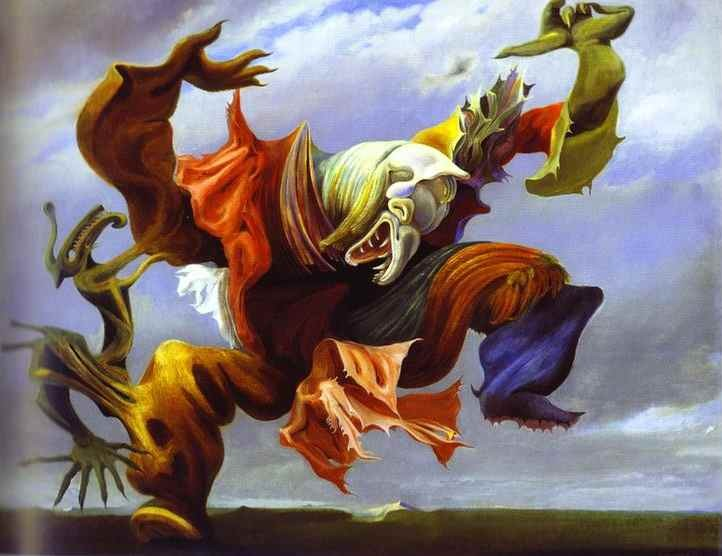
\includegraphics[width=0.4\textwidth]{imgs/ange0.jpg}}
\hspace{0.3cm}
\subfigure[Itération 1]{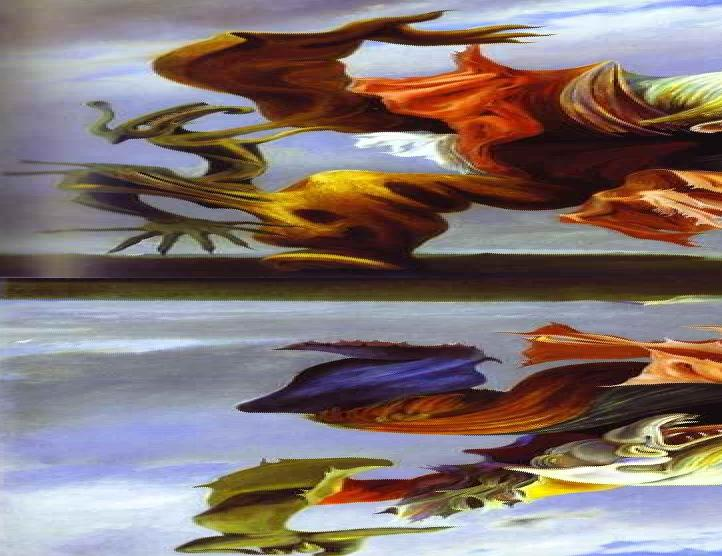
\includegraphics[width=0.4\textwidth]{imgs/ange1.jpg}}\\
\subfigure[Itération 2]{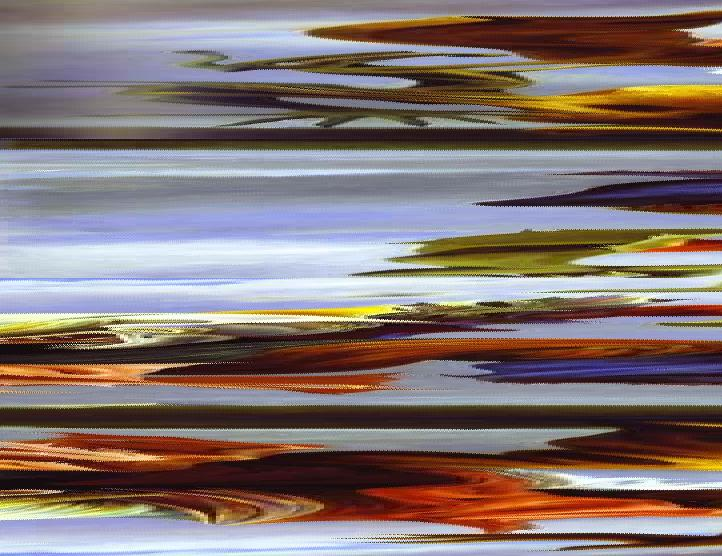
\includegraphics[width=0.4\textwidth]{imgs/ange2.jpg}}
\hspace{0.3cm}
\subfigure[Itération 100]{
\includegraphics[width=0.4\textwidth]{imgs/ange100.jpg}}
\end{figure}

\begin{itemize}
\item[\polygona] Justifier qu'en itérant la transformation on revient
  nécessairement en un nombre fini d'étapes sur l'image initiale.
\\Le nombre minimal d'étapes nécessaires pour revenir est
appelé \emph{temps de retour} et ne
dépend que des dimensions de l'image.
\item[\polygonb] En considérant la trajectoire de chaque pixel au fil des
  itérations, proposez un moyen simple d'exprimer le temps de retour
  d'une image. En déduire une façon rapide (linéaire en la taille de l'image) de
  le calculer.\\
  Implémentez cette méthode et calculez le temps de retour de votre image. Qu'en
  pensez-vous ?
\item[\polygonc] En déduire une méthode pour calculer la $n$\ieme{} itération de la transformation efficacement (en temps linéaire en la taille de l'image et indépendament de $n$, si l'on ignore la complexité arithmétique).
\item[\polygond] Vous avez maintenant toutes les clefs en main pour révéler l'image \texttt{Defi5/image.png} à l'aide des indices contenus dans le fichier \texttt{Defi5/indices.txt}. À vous de jouer\ldots{}
\end{itemize}

%%%%%%%  F  I  N  %%%%%%%%%%%%%%%
\label{lastpage}
\end{document}
